\section{Introduction}

%LIGO is getting bigger and better, and running into new noise sources as the noise floor drops. Other detectors with an even better low frequency sensitivity will have a lot to worry about with angular controls.
%
%Angular traps are interesting to study because they have a number of potential uses in controlling the motion of optical components. They have the advantage of a much lower minimum noise than conventional sensing methods. They have the potential to   
%
%we demonstrate a trap for a 0.4 gram mirror in the position and yaw degrees of freedom.


The Laser Interferometer Gravitational-wave Observatory (LIGO) is part of a world-wide 
effort to detect gravitational waves and use them to study the universe \cite{BPAbbott09}. Construction of 
LIGO's advanced detectors has finished and the first science runs will begin soon. The goal of Advanced LIGO (aLIGO) is the first direct detection of gravitational-waves 
from astrophysical sources such as coalescing compact binaries and core-collapse supernovae.
These detections will open a new spectrum for observing the universe and establish the field of 
gravitational-wave astronomy. 
These initial observations will also show the potential science gain of further increasing the state-of-the-art sensitivity of gravitational wave detectors \cite{Smith09,Harry10,Losurdo12}. Such detectors operate near the Standard Quantum Limit, meaning that the contributions from quantum radiation pressure and shot noise are about equal in the observation band \cite{Caves80, Ni86}.

To design a successor to aLIGO, techniques to operate gravitational-wave interferometers below 
the Standard Quantum Limit need to be developed \cite{Dan12, Chen13}. Dual carrier control systems and angular control 
using stable optical springs are promising methods for evading quantum-mechanical limitations on 
detector sensitivity \cite{LIGO10, Braginsky02b, Arcizet06b, Corbitt06b, Kippenberg05, Sheard04}. 
In 2007 Corbitt et al. at the LIGO Laboratory at the Massachusetts Institute of Technology 
demonstrated a one-dimensional optical trap of a one gram mirror using a novel two-carrier scheme \cite{Corbitt07}. 
%Although they did not completely turn off the low frequency feedback to the trapped mirror, 
Their work 
clearly demonstrated the potential of this technique. Extended to angular degrees of freedom, it has 
the prospect of opening a completely new approach to the angular control problem in future generation 
gravitational-wave detectors \cite{Punturo10}. 
Sidles and Sigg have shown that, for a Fabry-Perot cavity with a single 
resonating laser field, the radiation pressure force will couple the two end mirrors, always creating one 
soft (unstable) and one hard (stable) mode \cite{Sidles06}. This sets a lower limit on the required angular control 
bandwidth, which inevitably results in higher noise contamination by angular control noise and limits the angular control performance in the first and second generation 
gravitational-wave interferometers \cite{LIGO10, Braginsky01, Dooley13, Hirose10}. 
Angular optical trapping can bypass the Sidles-Sigg instability. Its fundamental noise limit is quantum radiation pressure noise, making it a promising candidate for low-noise angular control.


\section{Optical Springs}
In this paper, we will discuss the control of a mirror using two pairs of optical springs, creating two stable degrees of freedom in a single mirror. One pair will be a executed in a straight cavity and one will be in a folded cavity. In a previous paper, we have derived the behavior of a single optical spring in a straight cavity:

\begin{eqnarray}
\label{eq:KOSlong}
K_{OS} & {\approx} & P_0 t_1^2 \frac{8k}{c(1-r_1r_2)^3}\frac{ \frac{\delta}{\gamma}}{(1+\frac{\delta^2}{\gamma^2})} 
\frac{1}{1+\frac{\delta^2}{\gamma^2}-\frac{\Omega^2}{\gamma^2}+i2\frac{\Omega}{\gamma} }
\end{eqnarray}

In the appendix, we demonstrate the optical spring behavior of a folded cavity optical spring.
\begin{eqnarray}
\label{eq:KOSfolded}
K_{OS} & {\approx} & P_0 t_1^2 \frac{32k}{c(1-(r_1r_2)^2)^3}\frac{ \frac{\delta}{\gamma}}{(1+\frac{\delta^2}{\gamma^2})} 
\frac{1}{1+\frac{\delta^2}{\gamma^2}-\frac{\Omega^2}{\gamma^2}+i2\frac{\Omega}{\gamma} }
\end{eqnarray}

We note that the only differences between the two equations are a factor of four in the numerator and the change of $r_1r_2$ to $(r_1r_2)^2$ in the denominator.

Because these beams are exerting force on a single mirror, we expect some crosstalk between the straight optical spring pair and the folded optical spring pair. We have attempted to minimize this though our choice of spot locations on the mirror (see appendix \ref{ap:beamseparation}).


\section{Setup}
Our experiment (see fig. \ref{f:experimentLayout}) uses a 2 Watt 1064 nm Nd:YAG laser. The laser beam is split into a carrier beam and a subcarrier beam, then the subcarrier is frequency shifted by a tunable amount, described in more detail in section IV of our previous paper \cite{Kelley15}. The two beams are mode matched and spatially recombined (in opposite linear polarizations) in a Mach-Zehnder-style setup. The recombined beam is then split using an unpolarized beamsplitter into main and side beams. The main beam enters the straight cavity, while the side beam enters the folded cavity. Both polarizations of both beams are monitored in transmission and reflection.



\begin{table}[h]
\begin{tabular}{|l|l|l|}
\hline
Parameter & Straight & Folded \\ \hline
$\lambda_0$ & 1064 nm & 1064 nm \\ \hline
Mirror1,3,4 RoC & 7.5 cm & 7.5 cm \\ \hline
Mirror2 RoC & 5.0 cm & 5.0 cm \\ \hline
$L_0$ & 10.0 cm & 20.0 cm \\ \hline
M1,3,4 Spot size  & 268 $\mu$m & 268 $\mu$m\\ \hline
M2 Spot size  & 155 $\mu$m & 155 $\mu$m\\ \hline
FSR      & 1.50 GHz & 0.75 GHz \\ \hline
Finesse & 7500 & 3750 \\ \hline
Cavity Pole & 98.6 KHz & 98.6 KHz\\ \hline
Folded cavity angle, $\theta$ & 11 deg\\ \hline
\end{tabular}
%\end{table}
%
%\begin{table}[h]
\begin{tabular}{|l|l|}
\hline
$\delta f_{C}$ & 213-290 KHz \\ \hline
$\delta f_{SC}$ & 27-36 KHz \\ \hline
$P_{C}$ input& 225-239 mW \\ \hline
$P_{SC}$ input & 65-78 mW \\ \hline
\end{tabular}
\caption[Angular trap optical parameters]{Optical setup for the angular trap. The straight and folded cavities have different parameters due to the difference in total length and number of mirrors. RIGHT TABLE IS NONSENSE.}
\label{tab:longAngParams}
\end{table}


\begin{figure}[p]
\begin{center}
\includegraphics[width=.9\textwidth]{figures/Angular/simplifiedLayout}
\end{center}
\caption[Angular trap experiment layout]{%
\label{f:experimentLayout}
Layout of the angular trap cavity experiment.
The light from the laser is split into the carrier and subcarrier paths with a polarizing beam splitter (PBS), with a ratio determined by the $\lambda/2$ plate.
The subcarrier path is frequency shifted by two AOMs under the control of the subcarrier servo then recombined with the carrier with another PBS. 
The co-aligned mode-matched beams are then split into main and side paths, which enter the trap cavity.
The main beam has a straight optical path and is read out in transmission by broadband photodiodes and in reflection by RFPD1.
The side beam has a folded optical path and is read out in transmission by broadband photodiodes and in reflection by RFPD2.
We can use the 35 MHz modulation from the EOM with the two RFPDs in a PDH scheme to read out the cavity
lengths or lock the cavities.
}
\end{figure}


\section{Appendix}
To determine the behavior of a folded optical spring, we can compare it to the standard optical spring derivation \cite{Perreca14}.

We begin with a folded cavity with three mirrors, shown in fig. \ref{f:angularLayout}. We assume that M3 and M4 have the same amplitude reflectivity as M1, $r_1$, while we allow the end mirror to have a different reflectivity, $r_2$. The incoming field is $E=e^{\frac{i 2 \pi c t}{\lambda}}$. The average round-trip path length is $L = 2L_0$, where $L_0$ is the optical patch length between mirrors M3 and M4. We consider microscopic changes in cavity length $d_n$, which are discreet samples of a harmonic oscillation $d(t) =  x_0 e^{i\Omega t}$. The light travel time between M3 and M4 is $\tau = \frac{L_0}{c}$. It is important to note that the cavity length $L_0$ of the folded cavity is twice that of the straight cavity in our experiment.

\begin{figure}[p]
\vspace{5pt}
\begin{center}
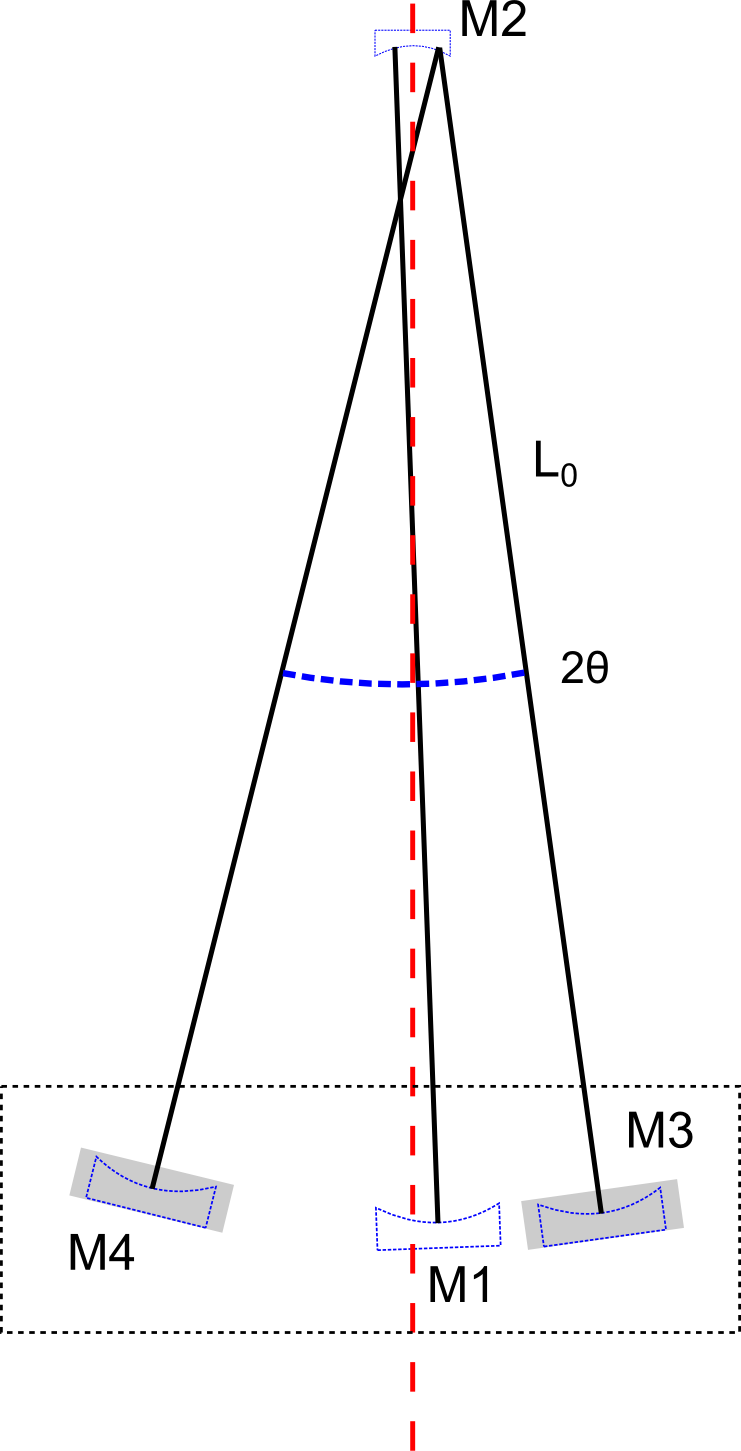
\includegraphics[width=.5\textwidth]{figures/Angular/angularLayout}
\end{center}
\caption[Folded cavity layout]{%
\label{f:angularLayout}
Layout of the angular trap cavity. Light enters through mirrors M1 and M3. The angle $\theta$ of the folded cavity is measured from the normal of M1. 
}
\end{figure}

We can use the same $X$ and $Y$ notation as the original derivation with one small change. $Y=e^{-i\Omega 2\tau}$ is the same, but now $X=(r_1r_2)^2 e^{\frac{-i2\pi L}{\lambda}}$ because the optical path touches M3 and M4 once and M2 twice.

We consider a set of displacements $d_n$, discretely sampled from a continuously oscilating function. This is equivelent to driving the cavity length at angular frequency $\Omega$.  
\begin{eqnarray}
d(t) = x_0e^{i \Omega(t-(2n-1)\tau)}\\
d_1 = x_0e^{i \Omega(t-\tau)}\\
d_n = Y^{2n-2}d_1  
\end{eqnarray}

Following \cite{Perreca14}, we get an equation for the electric field in the cavity, which we must change to reflect that we can only have real values for $d_1$.

\begin{eqnarray}
\label{e:Etot}
E_{tot} = \frac{t_1 E}{1-X}\left[ 1- \frac{4i\pi d_1}{\lambda}\frac{X}{1-Y^2X}\right]\nonumber\\
E_{tot} = \frac{t_1 E}{1-X}\left[ 1- \frac{4i\pi}{\lambda}\left(\frac{ d_1}{1-Y^2X}+\frac{ \overline{d}_1}{1-\overline{Y}^2X}\right)\right]
\end{eqnarray}

Then we get the cavity power:

\begin{eqnarray}
\label{e:P}
P&=&E_{tot}\cdot \overline{E}_{tot}=P_0 t^2\left[ \frac{i 2\pi Y}{\lambda(1-X)(1-\overline{X})}\left(\frac{X}{1-Y^2X}-\frac{\overline{X}}{1-Y^2\overline{X}}\right)\delta L+cc\right]  
%&-&\frac{ikX xY}{(1-\overline{X})(1-X)(1-Y^2 X)} -
%\frac{ikX \bar{x}\overline{Y}}{(1-\overline{X})(1-X)(1-\overline{Y}^2 X)}\nonumber \\
%&+&\frac{ik\overline{X} \bar{x}\overline{Y} } {(1-\overline{X})(1-X)(1-\overline{Y}^2 \overline{X})}+ 
%\frac{ik\overline{X} xY}{(1-\overline{X})(1-X)(1-Y^2 \overline{X})}]  \nonumber \\
%P &=&-P_0t^2 \left[ \frac{ikY}{(1-\overline{X})(1-X)} \left( \frac{X(1+Y^2)}{1-Y^2 X}-\frac{\overline{X}(1+\overline{Y}^2)}{1-Y^2\overline{X}} \right) x + cc \right]?
\end{eqnarray}

We add an extra $Y^{1/2}$ term to get to the other side of the cavity.
It is important to note that the change in cavity length $\delta L$ used here is strictly that: the cavity length. If we want to transpose that into longitudinal change, we need to multiply by a geometric factor (see fig. \ref{f:angularLayout}):

\begin{equation}
\delta L = \frac{2 \delta z}{\mbox{Cos}(\theta)}
\label{e:deltaL}
\end{equation}

There is similarly a geometric correction when calculating the radiation pressure force $F_{rad}$

\begin{eqnarray}
F_{rad} &=& \frac{2r_2^2}{c} P (2 \mbox{Cos}(\theta)) = K_z \delta z\\
&=& \frac{2r_2^2}{c} (2 \mbox{Cos}(\theta)) P_0 t^2\left[ \frac{i 2\pi Y^{3/2}}{\lambda(1-X)(1-\overline{X})}\left(\frac{X}{1-Y^2X}-\frac{\overline{X}}{1-Y^2\overline{X}}\right)\frac{2 \delta z}{\mbox{Cos}(\theta)}+cc\right] 
\label{e:Frad}
\end{eqnarray}

thus 
\begin{equation}
K_z=\frac{4r_2^2}{c} P_0 t^2 \frac{i 4\pi Y^{3/2}}{\lambda(1-X)(1-\overline{X})}\left(\frac{X}{1-Y^2X}-\frac{\overline{X}}{1-Y^2\overline{X}}\right)
\label{eq:Kz}
\end{equation}

With detuning:

\begin{equation}
X \rightarrow X=(r_1r_2)^2 e^{-i2\delta\tau}
\label{e:Xdet}
\end{equation}

Here $\delta = \omega_0-\omega_{res}$, the angular frequency detuning from the cavity resonance, $\omega_{res} = 2\pi n c/L$, and $\omega_0$ is the frequency of the laser.

\begin{eqnarray}
K_{OS}=&-P_0 t^2 r_2^2 \frac{16i\pi e^{-\frac{3}{2}i\Omega\tau}}{\lambda c(1-(r_1r_2)^2e^{i2\delta\tau})(1-(r_1r_2)^2e^{-i2\delta\tau})}\times\nonumber\\
 & \left( \frac{(r_1r_2)^2e^{-i\delta \tau}}{1-(r_1r_2)^2e^{-2i\Omega\tau} e^{-i2\delta\tau}}
 -\frac{(r_1r_2)^2e^{i2\delta\tau}}{1-(r_1r_2)^2e^{-2i\Omega\tau}e^{i2\delta\tau}} \right) 
\end{eqnarray}

Considering the finesse for the folded cavity to be $F = \pi\frac{FSR}{\gamma} \approx \frac{\pi}{1-(r_1r_2)^2} $

keep in mind that we have half the FSR of a non-folded cavity and half the finesse, so $\gamma$ is the same here as it is for the longitudinal trap.

\begin{eqnarray}
\label{eq:KOSfold}
K_{OS} & {\approx} & P_0 t_1^2 \frac{32k}{c(1-(r_1r_2)^2)^3}\frac{ \frac{\delta}{\gamma}}{(1+\frac{\delta^2}{\gamma^2})} 
\frac{1}{1+\frac{\delta^2}{\gamma^2}-\frac{\Omega^2}{\gamma^2}+i2\frac{\Omega}{\gamma} }
\end{eqnarray}

This is important because it means that a folded cavity angular spring will behave differently. Namely, the folded cavity spring constant is four times larger in magnitude than a similar straight cavity, and there is a change of $r_1r_2$ to $(r_1r_2)^2$.

\subsection{angular issues}
worried about the change in beam shape
not an issue (but did lock on TEM01)
\begin{figure}[htp]%
\begin{center}
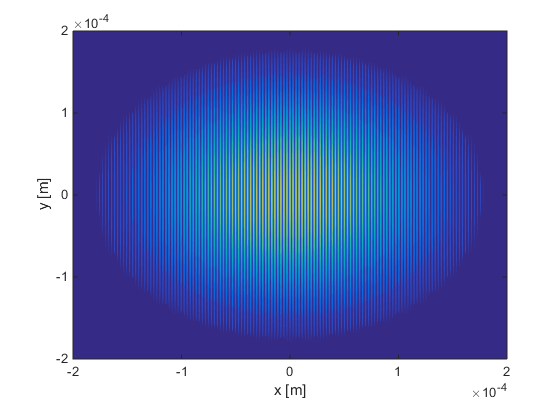
\includegraphics[width=.8\textwidth]{figures/Angular/11deginterference}%lab\lab2014\OpticalLayout\20140903_angular_options
\caption[Folded cavity interference pattern]{Simulated folded cavity interference pattern on the surface of M2. This corresponds to the power deposited into the mirror and thus the amplitude of the photothermal effect. Using this and the diffusion length as a function of frequency, we showed that there would be no significant amplification of the photothermal effect due to this distribution of absorbed power.}%
\end{center}
\label{fig:foldedinterference}%
\end{figure}

shape of power distribution on end mirror.
